\documentclass[1p]{elsarticle_modified}
%\bibliographystyle{elsarticle-num}

%\usepackage[colorlinks]{hyperref}
%\usepackage{abbrmath_seonhwa} %\Abb, \Ascr, \Acal ,\Abf, \Afrak
\usepackage{amsfonts}
\usepackage{amssymb}
\usepackage{amsmath}
\usepackage{amsthm}
\usepackage{scalefnt}
\usepackage{amsbsy}
\usepackage{kotex}
\usepackage{caption}
\usepackage{subfig}
\usepackage{color}
\usepackage{graphicx}
\usepackage{xcolor} %% white, black, red, green, blue, cyan, magenta, yellow
\usepackage{float}
\usepackage{setspace}
\usepackage{hyperref}

\usepackage{tikz}
\usetikzlibrary{arrows}

\usepackage{multirow}
\usepackage{array} % fixed length table
\usepackage{hhline}

%%%%%%%%%%%%%%%%%%%%%
\makeatletter
\renewcommand*\env@matrix[1][\arraystretch]{%
	\edef\arraystretch{#1}%
	\hskip -\arraycolsep
	\let\@ifnextchar\new@ifnextchar
	\array{*\c@MaxMatrixCols c}}
\makeatother %https://tex.stackexchange.com/questions/14071/how-can-i-increase-the-line-spacing-in-a-matrix
%%%%%%%%%%%%%%%

\usepackage[normalem]{ulem}

\newcommand{\msout}[1]{\ifmmode\text{\sout{\ensuremath{#1}}}\else\sout{#1}\fi}
%SOURCE: \msout is \stkout macro in https://tex.stackexchange.com/questions/20609/strikeout-in-math-mode

\newcommand{\cancel}[1]{
	\ifmmode
	{\color{red}\msout{#1}}
	\else
	{\color{red}\sout{#1}}
	\fi
}

\newcommand{\add}[1]{
	{\color{blue}\uwave{#1}}
}

\newcommand{\replace}[2]{
	\ifmmode
	{\color{red}\msout{#1}}{\color{blue}\uwave{#2}}
	\else
	{\color{red}\sout{#1}}{\color{blue}\uwave{#2}}
	\fi
}

\newcommand{\Sol}{\mathcal{S}} %segment
\newcommand{\D}{D} %diagram
\newcommand{\A}{\mathcal{A}} %arc


%%%%%%%%%%%%%%%%%%%%%%%%%%%%%5 test

\def\sl{\operatorname{\textup{SL}}(2,\Cbb)}
\def\psl{\operatorname{\textup{PSL}}(2,\Cbb)}
\def\quan{\mkern 1mu \triangleright \mkern 1mu}

\theoremstyle{definition}
\newtheorem{thm}{Theorem}[section]
\newtheorem{prop}[thm]{Proposition}
\newtheorem{lem}[thm]{Lemma}
\newtheorem{ques}[thm]{Question}
\newtheorem{cor}[thm]{Corollary}
\newtheorem{defn}[thm]{Definition}
\newtheorem{exam}[thm]{Example}
\newtheorem{rmk}[thm]{Remark}
\newtheorem{alg}[thm]{Algorithm}

\newcommand{\I}{\sqrt{-1}}
\begin{document}

%\begin{frontmatter}
%
%\title{Boundary parabolic representations of knots up to 8 crossings}
%
%%% Group authors per affiliation:
%\author{Yunhi Cho} 
%\address{Department of Mathematics, University of Seoul, Seoul, Korea}
%\ead{yhcho@uos.ac.kr}
%
%
%\author{Seonhwa Kim} %\fnref{s_kim}}
%\address{Center for Geometry and Physics, Institute for Basic Science, Pohang, 37673, Korea}
%\ead{ryeona17@ibs.re.kr}
%
%\author{Hyuk Kim}
%\address{Department of Mathematical Sciences, Seoul National University, Seoul 08826, Korea}
%\ead{hyukkim@snu.ac.kr}
%
%\author{Seokbeom Yoon}
%\address{Department of Mathematical Sciences, Seoul National University, Seoul, 08826,  Korea}
%\ead{sbyoon15@snu.ac.kr}
%
%\begin{abstract}
%We find all boundary parabolic representation of knots up to 8 crossings.
%
%\end{abstract}
%\begin{keyword}
%    \MSC[2010] 57M25 
%\end{keyword}
%
%\end{frontmatter}

%\linenumbers
%\tableofcontents
%
\newcommand\colored[1]{\textcolor{white}{\rule[-0.35ex]{0.8em}{1.4ex}}\kern-0.8em\color{red} #1}%
%\newcommand\colored[1]{\textcolor{white}{ #1}\kern-2.17ex	\textcolor{white}{ #1}\kern-1.81ex	\textcolor{white}{ #1}\kern-2.15ex\color{red}#1	}

{\Large $\underline{10_{86}~(K10a_{84})}$}

\setlength{\tabcolsep}{10pt}
\renewcommand{\arraystretch}{1.6}
\vspace{1cm}\begin{tabular}{m{100pt}>{\centering\arraybackslash}m{274pt}}
\multirow{5}{120pt}{
	\centering
	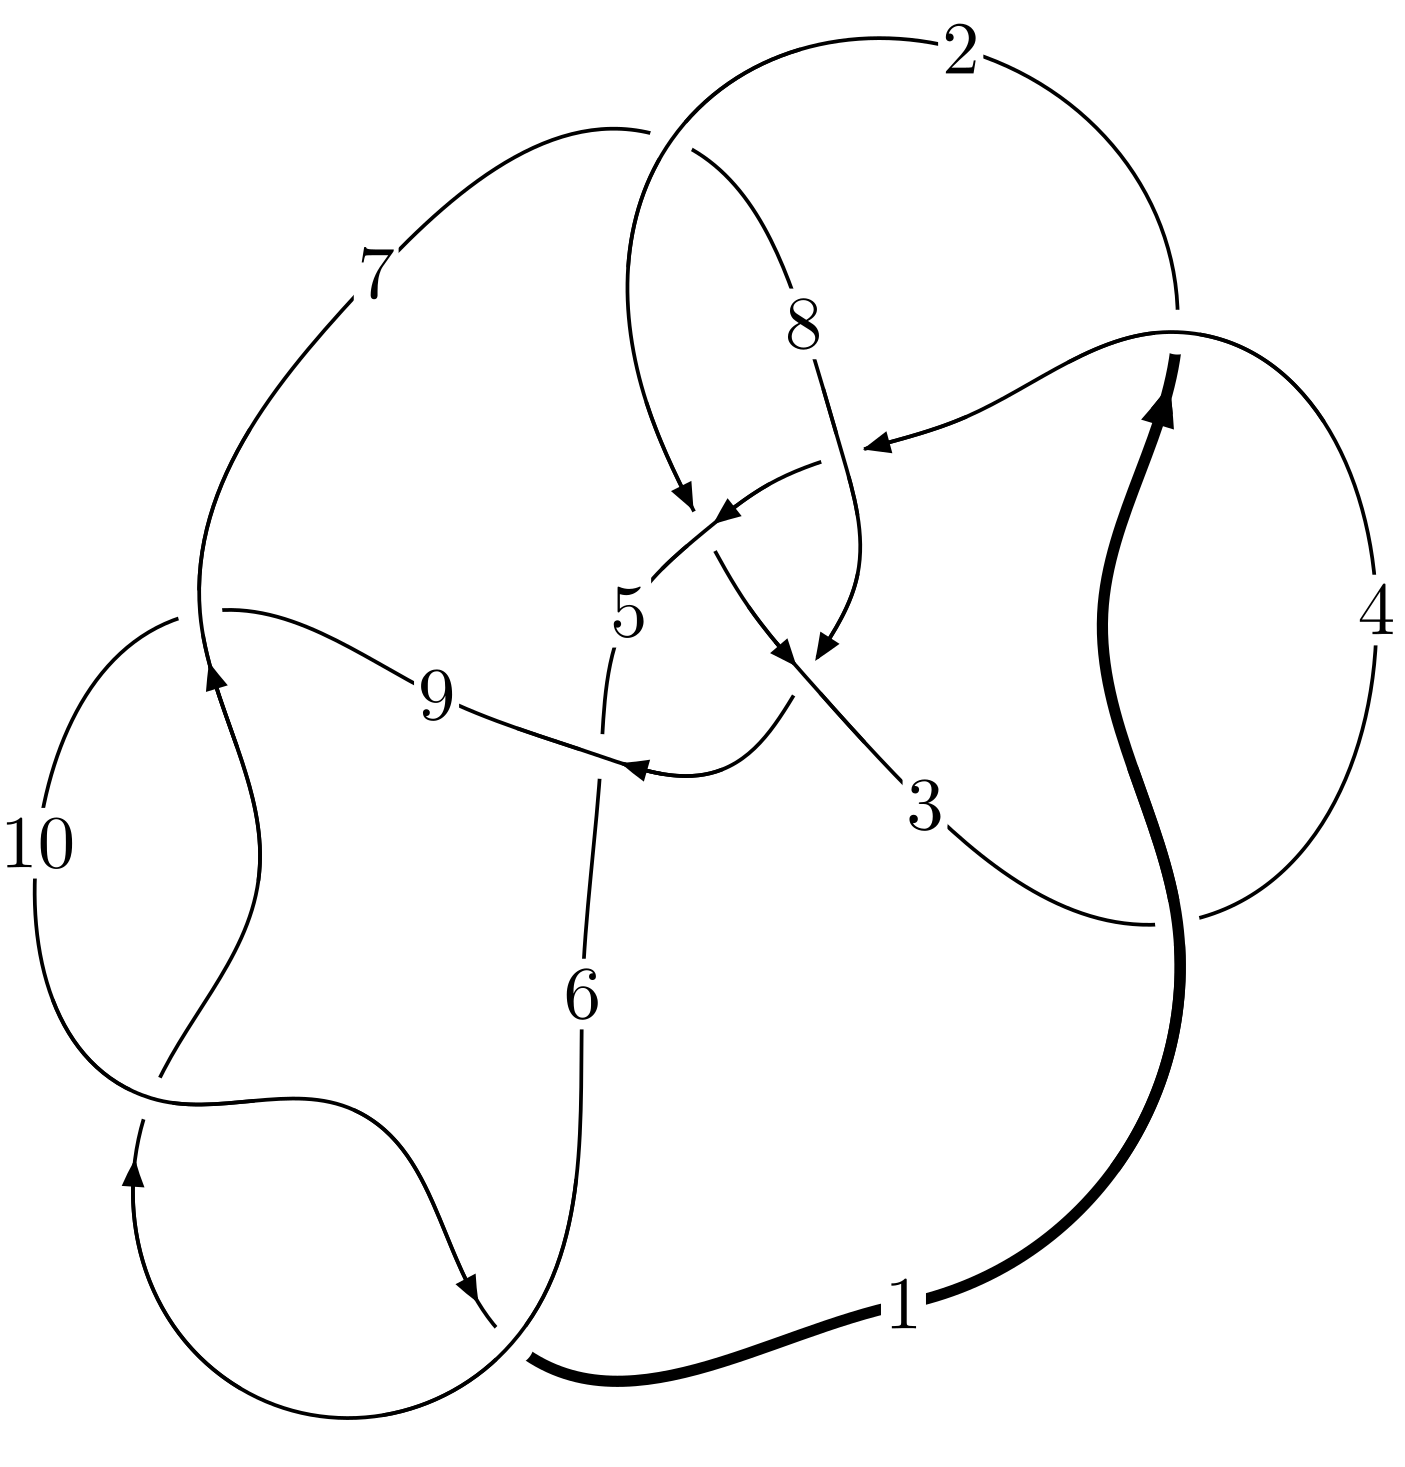
\includegraphics[width=112pt]{../../../GIT/diagram.site/Diagrams/png/170_10_86.png}\\
\ \ \ A knot diagram\footnotemark}&
\allowdisplaybreaks
\textbf{Linearized knot diagam} \\
\cline{2-2}
 &
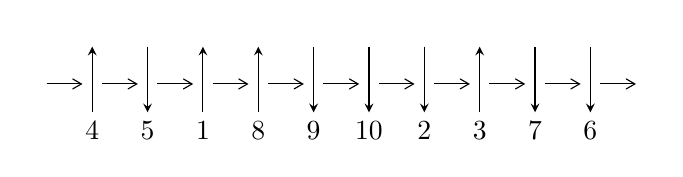
\begin{tikzpicture}[x=20pt, y=17pt]
	% nodes
	\node (C0) at (0, 0) {};
	\node (C1) at (1, 0) {};
	\node (C1U) at (1, +1) {};
	\node (C1D) at (1, -1) {4};

	\node (C2) at (2, 0) {};
	\node (C2U) at (2, +1) {};
	\node (C2D) at (2, -1) {5};

	\node (C3) at (3, 0) {};
	\node (C3U) at (3, +1) {};
	\node (C3D) at (3, -1) {1};

	\node (C4) at (4, 0) {};
	\node (C4U) at (4, +1) {};
	\node (C4D) at (4, -1) {8};

	\node (C5) at (5, 0) {};
	\node (C5U) at (5, +1) {};
	\node (C5D) at (5, -1) {9};

	\node (C6) at (6, 0) {};
	\node (C6U) at (6, +1) {};
	\node (C6D) at (6, -1) {10};

	\node (C7) at (7, 0) {};
	\node (C7U) at (7, +1) {};
	\node (C7D) at (7, -1) {2};

	\node (C8) at (8, 0) {};
	\node (C8U) at (8, +1) {};
	\node (C8D) at (8, -1) {3};

	\node (C9) at (9, 0) {};
	\node (C9U) at (9, +1) {};
	\node (C9D) at (9, -1) {7};

	\node (C10) at (10, 0) {};
	\node (C10U) at (10, +1) {};
	\node (C10D) at (10, -1) {6};
	\node (C11) at (11, 0) {};

	% arrows
	\draw[->,>={angle 60}]
	(C0) edge (C1) (C1) edge (C2) (C2) edge (C3) (C3) edge (C4) (C4) edge (C5) (C5) edge (C6) (C6) edge (C7) (C7) edge (C8) (C8) edge (C9) (C9) edge (C10) (C10) edge (C11) ;	\draw[->,>=stealth]
	(C1D) edge (C1U) (C2U) edge (C2D) (C3D) edge (C3U) (C4D) edge (C4U) (C5U) edge (C5D) (C6U) edge (C6D) (C7U) edge (C7D) (C8D) edge (C8U) (C9U) edge (C9D) (C10U) edge (C10D) ;
	\end{tikzpicture} \\
\hhline{~~} \\& 
\textbf{Solving Sequence} \\ \cline{2-2} 
 &
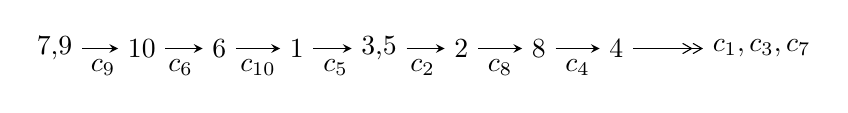
\begin{tikzpicture}[x=28pt, y=7pt]
	% node
	\node (A0) at (-1/8, 0) {7,9};
	\node (A1) at (1, 0) {10};
	\node (A2) at (2, 0) {6};
	\node (A3) at (3, 0) {1};
	\node (A4) at (65/16, 0) {3,5};
	\node (A5) at (41/8, 0) {2};
	\node (A6) at (49/8, 0) {8};
	\node (A7) at (57/8, 0) {4};
	\node (C1) at (1/2, -1) {$c_{9}$};
	\node (C2) at (3/2, -1) {$c_{6}$};
	\node (C3) at (5/2, -1) {$c_{10}$};
	\node (C4) at (7/2, -1) {$c_{5}$};
	\node (C5) at (37/8, -1) {$c_{2}$};
	\node (C6) at (45/8, -1) {$c_{8}$};
	\node (C7) at (53/8, -1) {$c_{4}$};
	\node (A8) at (9, 0) {$c_{1},c_{3},c_{7}$};

	% edge
	\draw[->,>=stealth]	
	(A0) edge (A1) (A1) edge (A2) (A2) edge (A3) (A3) edge (A4) (A4) edge (A5) (A5) edge (A6) (A6) edge (A7) ;
	\draw[->>,>={angle 60}]	
	(A7) edge (A8);
\end{tikzpicture} \\ 

\end{tabular} \\

\footnotetext{
The image of knot diagram is generated by the software ``\textbf{Draw programme}" developed by Andrew Bartholomew(\url{http://www.layer8.co.uk/maths/draw/index.htm\#Running-draw}), where we modified some parts for our purpose(\url{https://github.com/CATsTAILs/LinksPainter}).
}\phantom \\ \newline 
\centering \textbf{Ideals for irreducible components\footnotemark of $X_{\text{par}}$} 
 
\begin{align*}
I^u_{1}&=\langle 
-4039601920 u^{41}+442991781120 u^{40}+\cdots+60302773206589 b+12060836,\\
\phantom{I^u_{1}}&\phantom{= \langle  }317833596 u^{41}-21861098876 u^{40}+\cdots+60302773206589 a+110555084616603,\\
\phantom{I^u_{1}}&\phantom{= \langle  }u^{42}- u^{41}+\cdots-3 u+1\rangle \\
\\
\end{align*}
\raggedright * 1 irreducible components of $\dim_{\mathbb{C}}=0$, with total 42 representations.\\
\footnotetext{All coefficients of polynomials are rational numbers. But the coefficients are sometimes approximated in decimal forms when there is not enough margin.}
\newpage
\renewcommand{\arraystretch}{1}
\centering \section*{I. $I^u_{1}= \langle -4.04\times10^{9} u^{41}+4.43\times10^{11} u^{40}+\cdots+6.03\times10^{13} b+1.21\times10^{7},\;3.18\times10^{8} u^{41}-2.19\times10^{10} u^{40}+\cdots+6.03\times10^{13} a+1.11\times10^{14},\;u^{42}- u^{41}+\cdots-3 u+1 \rangle$}
\flushleft \textbf{(i) Arc colorings}\\
\begin{tabular}{m{7pt} m{180pt} m{7pt} m{180pt} }
\flushright $a_{7}=$&$\begin{pmatrix}0\\u\end{pmatrix}$ \\
\flushright $a_{9}=$&$\begin{pmatrix}1\\0\end{pmatrix}$ \\
\flushright $a_{10}=$&$\begin{pmatrix}1\\u^2\end{pmatrix}$ \\
\flushright $a_{6}=$&$\begin{pmatrix}u\\u^3+u\end{pmatrix}$ \\
\flushright $a_{1}=$&$\begin{pmatrix}u^2+1\\u^4+2 u^2\end{pmatrix}$ \\
\flushright $a_{3}=$&$\begin{pmatrix}-5.27063\times10^{-6} u^{41}+0.000362522 u^{40}+\cdots+5.66153 u-1.83333\\0.0000669887 u^{41}-0.00734613 u^{40}+\cdots+3.16667 u-2.00005\times10^{-7}\end{pmatrix}$ \\
\flushright $a_{5}=$&$\begin{pmatrix}u^3+2 u\\u^3+u\end{pmatrix}$ \\
\flushright $a_{2}=$&$\begin{pmatrix}6.83829\times10^{-7} u^{41}-0.0000369667 u^{40}+\cdots+5.57750 u-1.75000\\0.000767581 u^{41}-0.0917794 u^{40}+\cdots+3.25001 u-3.08389\times10^{-6}\end{pmatrix}$ \\
\flushright $a_{8}=$&$\begin{pmatrix}0.00250009 u^{41}-0.00247925 u^{40}+\cdots+5.08221 u-0.722479\\0.0000486247 u^{41}-0.00588236 u^{40}+\cdots+3.33172 u-0.00583354\end{pmatrix}$ \\
\flushright $a_{4}=$&$\begin{pmatrix}-1.19089\times10^{-6} u^{41}+0.0000798978 u^{40}+\cdots+6.41681 u-1.01667\\-0.000140118 u^{41}+0.0168866 u^{40}+\cdots+3.18333 u+5.76776\times10^{-7}\end{pmatrix}$\\&\end{tabular}
\flushleft \textbf{(ii) Obstruction class $= -1$}\\~\\
\flushleft \textbf{(iii) Cusp Shapes $= \frac{191762525603096}{60302773206589} u^{41}-\frac{143500206823500}{60302773206589} u^{40}+\cdots-\frac{332549985427516}{60302773206589} u+\frac{276206801861070}{60302773206589}$}\\~\\
\newpage\renewcommand{\arraystretch}{1}
\flushleft \textbf{(iv) u-Polynomials at the component}\newline \\
\begin{tabular}{m{50pt}|m{274pt}}
Crossings & \hspace{64pt}u-Polynomials at each crossing \\
\hline $$\begin{aligned}c_{1},c_{3}\end{aligned}$$&$\begin{aligned}
&u^{42}+u^{41}+\cdots+7 u+1
\end{aligned}$\\
\hline $$\begin{aligned}c_{2}\end{aligned}$$&$\begin{aligned}
&u^{42}-7 u^{41}+\cdots- u+1
\end{aligned}$\\
\hline $$\begin{aligned}c_{4}\end{aligned}$$&$\begin{aligned}
&u^{42}-3 u^{41}+\cdots- u+1
\end{aligned}$\\
\hline $$\begin{aligned}c_{5}\end{aligned}$$&$\begin{aligned}
&u^{42}+u^{41}+\cdots+37 u+17
\end{aligned}$\\
\hline $$\begin{aligned}c_{6},c_{9},c_{10}\end{aligned}$$&$\begin{aligned}
&u^{42}- u^{41}+\cdots-3 u+1
\end{aligned}$\\
\hline $$\begin{aligned}c_{7}\end{aligned}$$&$\begin{aligned}
&u^{42}- u^{41}+\cdots-10 u+4
\end{aligned}$\\
\hline $$\begin{aligned}c_{8}\end{aligned}$$&$\begin{aligned}
&u^{42}+u^{41}+\cdots+21 u+1
\end{aligned}$\\
\hline
\end{tabular}\\~\\
\newpage\renewcommand{\arraystretch}{1}
\flushleft \textbf{(v) Riley Polynomials at the component}\newline \\
\begin{tabular}{m{50pt}|m{274pt}}
Crossings & \hspace{64pt}Riley Polynomials at each crossing \\
\hline $$\begin{aligned}c_{1},c_{3}\end{aligned}$$&$\begin{aligned}
&y^{42}-27 y^{41}+\cdots-7 y+1
\end{aligned}$\\
\hline $$\begin{aligned}c_{2}\end{aligned}$$&$\begin{aligned}
&y^{42}-3 y^{41}+\cdots-7 y+1
\end{aligned}$\\
\hline $$\begin{aligned}c_{4}\end{aligned}$$&$\begin{aligned}
&y^{42}-7 y^{41}+\cdots-3 y+1
\end{aligned}$\\
\hline $$\begin{aligned}c_{5}\end{aligned}$$&$\begin{aligned}
&y^{42}-7 y^{41}+\cdots-1539 y+289
\end{aligned}$\\
\hline $$\begin{aligned}c_{6},c_{9},c_{10}\end{aligned}$$&$\begin{aligned}
&y^{42}+37 y^{41}+\cdots-3 y+1
\end{aligned}$\\
\hline $$\begin{aligned}c_{7}\end{aligned}$$&$\begin{aligned}
&y^{42}+41 y^{41}+\cdots+308 y+16
\end{aligned}$\\
\hline $$\begin{aligned}c_{8}\end{aligned}$$&$\begin{aligned}
&y^{42}+33 y^{41}+\cdots-247 y+1
\end{aligned}$\\
\hline
\end{tabular}\\~\\
\newpage\flushleft \textbf{(vi) Complex Volumes and Cusp Shapes}
$$\begin{array}{c|c|c}  
\text{Solutions to }I^u_{1}& \I (\text{vol} + \sqrt{-1}CS) & \text{Cusp shape}\\
 \hline 
\begin{aligned}
u &= \phantom{-}0.478429 + 0.830661 I \\
a &= -1.016150 - 0.087138 I \\
b &= -0.936087 - 0.907522 I\end{aligned}
 & \phantom{-}2.62044 + 5.77796 I & \phantom{-}0.70723 - 3.77194 I \\ \hline\begin{aligned}
u &= \phantom{-}0.478429 - 0.830661 I \\
a &= -1.016150 + 0.087138 I \\
b &= -0.936087 + 0.907522 I\end{aligned}
 & \phantom{-}2.62044 - 5.77796 I & \phantom{-}0.70723 + 3.77194 I \\ \hline\begin{aligned}
u &= \phantom{-}0.185781 + 1.025770 I \\
a &= \phantom{-}0.077705 + 0.573452 I \\
b &= \phantom{-}0.483603 + 0.963768 I\end{aligned}
 & -0.411802 + 1.015420 I & -3.47498 - 1.21296 I \\ \hline\begin{aligned}
u &= \phantom{-}0.185781 - 1.025770 I \\
a &= \phantom{-}0.077705 - 0.573452 I \\
b &= \phantom{-}0.483603 - 0.963768 I\end{aligned}
 & -0.411802 - 1.015420 I & -3.47498 + 1.21296 I \\ \hline\begin{aligned}
u &= -0.850313\phantom{ +0.000000I} \\
a &= \phantom{-}0.302339\phantom{ +0.000000I} \\
b &= -0.0653539\phantom{ +0.000000I}\end{aligned}
 & -1.60575\phantom{ +0.000000I} & -10.6730\phantom{ +0.000000I} \\ \hline\begin{aligned}
u &= -0.750438 + 0.396807 I \\
a &= -0.358825 + 1.086560 I \\
b &= \phantom{-}0.176374 + 0.822398 I\end{aligned}
 & -0.84767 + 2.24209 I & -7.43868 - 8.38261 I \\ \hline\begin{aligned}
u &= -0.750438 - 0.396807 I \\
a &= -0.358825 - 1.086560 I \\
b &= \phantom{-}0.176374 - 0.822398 I\end{aligned}
 & -0.84767 - 2.24209 I & -7.43868 + 8.38261 I \\ \hline\begin{aligned}
u &= \phantom{-}0.798010 + 0.277511 I \\
a &= \phantom{-}0.55497 - 2.07637 I \\
b &= \phantom{-}1.12925 - 1.11829 I\end{aligned}
 & \phantom{-}0.84307 - 10.28750 I & -1.70761 + 7.71466 I \\ \hline\begin{aligned}
u &= \phantom{-}0.798010 - 0.277511 I \\
a &= \phantom{-}0.55497 + 2.07637 I \\
b &= \phantom{-}1.12925 + 1.11829 I\end{aligned}
 & \phantom{-}0.84307 + 10.28750 I & -1.70761 - 7.71466 I \\ \hline\begin{aligned}
u &= -0.439352 + 1.081720 I \\
a &= -0.241896 - 0.303592 I \\
b &= -0.301740 - 0.507276 I\end{aligned}
 & \phantom{-}1.66550 + 4.60168 I & -2.00000 - 9.10658 I\\
 \hline 
 \end{array}$$\newpage$$\begin{array}{c|c|c}  
\text{Solutions to }I^u_{1}& \I (\text{vol} + \sqrt{-1}CS) & \text{Cusp shape}\\
 \hline 
\begin{aligned}
u &= -0.439352 - 1.081720 I \\
a &= -0.241896 + 0.303592 I \\
b &= -0.301740 + 0.507276 I\end{aligned}
 & \phantom{-}1.66550 - 4.60168 I & -2.00000 + 9.10658 I \\ \hline\begin{aligned}
u &= \phantom{-}0.711781 + 0.186271 I \\
a &= \phantom{-}0.15739 + 1.81871 I \\
b &= -0.778762 + 0.849850 I\end{aligned}
 & -2.84345 - 4.53919 I & -5.58452 + 6.45237 I \\ \hline\begin{aligned}
u &= \phantom{-}0.711781 - 0.186271 I \\
a &= \phantom{-}0.15739 - 1.81871 I \\
b &= -0.778762 - 0.849850 I\end{aligned}
 & -2.84345 + 4.53919 I & -5.58452 - 6.45237 I \\ \hline\begin{aligned}
u &= -0.716527\phantom{ +0.000000I} \\
a &= -0.397959\phantom{ +0.000000I} \\
b &= -0.516879\phantom{ +0.000000I}\end{aligned}
 & -1.70188\phantom{ +0.000000I} & -6.91450\phantom{ +0.000000I} \\ \hline\begin{aligned}
u &= -0.160940 + 1.289060 I \\
a &= \phantom{-}1.70867 - 0.62606 I \\
b &= -0.56110 - 1.54770 I\end{aligned}
 & \phantom{-}4.17623 + 2.06372 I & \phantom{-0.000000 } 0 \\ \hline\begin{aligned}
u &= -0.160940 - 1.289060 I \\
a &= \phantom{-}1.70867 + 0.62606 I \\
b &= -0.56110 + 1.54770 I\end{aligned}
 & \phantom{-}4.17623 - 2.06372 I & \phantom{-0.000000 } 0 \\ \hline\begin{aligned}
u &= \phantom{-}0.088609 + 1.323910 I \\
a &= \phantom{-}1.12700 + 0.86778 I \\
b &= -0.377923 - 0.176136 I\end{aligned}
 & \phantom{-}4.85107 + 1.20148 I & \phantom{-0.000000 } 0 \\ \hline\begin{aligned}
u &= \phantom{-}0.088609 - 1.323910 I \\
a &= \phantom{-}1.12700 - 0.86778 I \\
b &= -0.377923 + 0.176136 I\end{aligned}
 & \phantom{-}4.85107 - 1.20148 I & \phantom{-0.000000 } 0 \\ \hline\begin{aligned}
u &= -0.279867 + 1.317280 I \\
a &= -0.218311 + 0.692861 I \\
b &= \phantom{-}0.843176 + 0.035564 I\end{aligned}
 & \phantom{-}2.51211 + 3.57467 I & \phantom{-0.000000 } 0 \\ \hline\begin{aligned}
u &= -0.279867 - 1.317280 I \\
a &= -0.218311 - 0.692861 I \\
b &= \phantom{-}0.843176 - 0.035564 I\end{aligned}
 & \phantom{-}2.51211 - 3.57467 I & \phantom{-0.000000 } 0\\
 \hline 
 \end{array}$$\newpage$$\begin{array}{c|c|c}  
\text{Solutions to }I^u_{1}& \I (\text{vol} + \sqrt{-1}CS) & \text{Cusp shape}\\
 \hline 
\begin{aligned}
u &= -0.215944 + 1.336170 I \\
a &= -2.06558 + 0.80088 I \\
b &= -0.18914 + 3.23351 I\end{aligned}
 & \phantom{-}4.98903 + 3.19900 I & \phantom{-0.000000 } 0 \\ \hline\begin{aligned}
u &= -0.215944 - 1.336170 I \\
a &= -2.06558 - 0.80088 I \\
b &= -0.18914 - 3.23351 I\end{aligned}
 & \phantom{-}4.98903 - 3.19900 I & \phantom{-0.000000 } 0 \\ \hline\begin{aligned}
u &= \phantom{-}0.173241 + 1.368420 I \\
a &= \phantom{-}0.844181 - 0.077998 I \\
b &= -1.145210 - 0.270649 I\end{aligned}
 & \phantom{-}7.73393 - 1.79873 I & \phantom{-0.000000 } 0 \\ \hline\begin{aligned}
u &= \phantom{-}0.173241 - 1.368420 I \\
a &= \phantom{-}0.844181 + 0.077998 I \\
b &= -1.145210 + 0.270649 I\end{aligned}
 & \phantom{-}7.73393 + 1.79873 I & \phantom{-0.000000 } 0 \\ \hline\begin{aligned}
u &= \phantom{-}0.228890 + 1.375810 I \\
a &= -0.37491 - 1.62208 I \\
b &= \phantom{-}0.514507 - 0.525372 I\end{aligned}
 & \phantom{-}6.95368 - 5.70185 I & \phantom{-0.000000 } 0 \\ \hline\begin{aligned}
u &= \phantom{-}0.228890 - 1.375810 I \\
a &= -0.37491 + 1.62208 I \\
b &= \phantom{-}0.514507 + 0.525372 I\end{aligned}
 & \phantom{-}6.95368 + 5.70185 I & \phantom{-0.000000 } 0 \\ \hline\begin{aligned}
u &= \phantom{-}0.563419 + 0.218408 I \\
a &= -0.72689 + 2.25592 I \\
b &= -0.451451 + 0.210468 I\end{aligned}
 & \phantom{-}1.89435 - 2.76342 I & \phantom{-}1.45970 + 7.65568 I \\ \hline\begin{aligned}
u &= \phantom{-}0.563419 - 0.218408 I \\
a &= -0.72689 - 2.25592 I \\
b &= -0.451451 - 0.210468 I\end{aligned}
 & \phantom{-}1.89435 + 2.76342 I & \phantom{-}1.45970 - 7.65568 I \\ \hline\begin{aligned}
u &= \phantom{-}0.286750 + 1.370360 I \\
a &= -1.21599 - 1.04777 I \\
b &= \phantom{-}0.946396 - 0.760155 I\end{aligned}
 & \phantom{-}2.08911 - 8.16087 I & \phantom{-0.000000 } 0 \\ \hline\begin{aligned}
u &= \phantom{-}0.286750 - 1.370360 I \\
a &= -1.21599 + 1.04777 I \\
b &= \phantom{-}0.946396 + 0.760155 I\end{aligned}
 & \phantom{-}2.08911 + 8.16087 I & \phantom{-0.000000 } 0\\
 \hline 
 \end{array}$$\newpage$$\begin{array}{c|c|c}  
\text{Solutions to }I^u_{1}& \I (\text{vol} + \sqrt{-1}CS) & \text{Cusp shape}\\
 \hline 
\begin{aligned}
u &= -0.553872 + 0.081016 I \\
a &= -0.34407 - 5.14524 I \\
b &= -0.19417 - 2.58841 I\end{aligned}
 & \phantom{-}0.484443 + 0.387619 I & \phantom{-}2.4374 + 16.9357 I \\ \hline\begin{aligned}
u &= -0.553872 - 0.081016 I \\
a &= -0.34407 + 5.14524 I \\
b &= -0.19417 + 2.58841 I\end{aligned}
 & \phantom{-}0.484443 - 0.387619 I & \phantom{-}2.4374 - 16.9357 I \\ \hline\begin{aligned}
u &= \phantom{-}0.32193 + 1.42127 I \\
a &= \phantom{-}0.86794 + 1.40076 I \\
b &= -1.30679 + 1.17931 I\end{aligned}
 & \phantom{-}6.2544 - 14.3413 I & \phantom{-0.000000 } 0 \\ \hline\begin{aligned}
u &= \phantom{-}0.32193 - 1.42127 I \\
a &= \phantom{-}0.86794 - 1.40076 I \\
b &= -1.30679 - 1.17931 I\end{aligned}
 & \phantom{-}6.2544 + 14.3413 I & \phantom{-0.000000 } 0 \\ \hline\begin{aligned}
u &= -0.180411 + 0.503978 I \\
a &= -0.786744 + 0.412670 I \\
b &= \phantom{-}0.291024 + 0.725866 I\end{aligned}
 & -0.258833 + 1.342430 I & -2.96321 - 4.26706 I \\ \hline\begin{aligned}
u &= -0.180411 - 0.503978 I \\
a &= -0.786744 - 0.412670 I \\
b &= \phantom{-}0.291024 - 0.725866 I\end{aligned}
 & -0.258833 - 1.342430 I & -2.96321 + 4.26706 I \\ \hline\begin{aligned}
u &= -0.31335 + 1.45744 I \\
a &= \phantom{-}0.573180 - 0.672710 I \\
b &= -0.502148 - 0.851645 I\end{aligned}
 & \phantom{-}5.06478 + 6.18924 I & \phantom{-0.000000 } 0 \\ \hline\begin{aligned}
u &= -0.31335 - 1.45744 I \\
a &= \phantom{-}0.573180 + 0.672710 I \\
b &= -0.502148 + 0.851645 I\end{aligned}
 & \phantom{-}5.06478 - 6.18924 I & \phantom{-0.000000 } 0 \\ \hline\begin{aligned}
u &= \phantom{-}0.02848 + 1.50835 I \\
a &= -0.206650 - 0.321775 I \\
b &= \phantom{-}1.154670 + 0.425800 I\end{aligned}
 & \phantom{-}10.43310 + 4.60033 I & \phantom{-0.000000 } 0 \\ \hline\begin{aligned}
u &= \phantom{-}0.02848 - 1.50835 I \\
a &= -0.206650 + 0.321775 I \\
b &= \phantom{-}1.154670 - 0.425800 I\end{aligned}
 & \phantom{-}10.43310 - 4.60033 I & \phantom{-0.000000 } 0\\
 \hline 
 \end{array}$$\newpage$$\begin{array}{c|c|c}  
\text{Solutions to }I^u_{1}& \I (\text{vol} + \sqrt{-1}CS) & \text{Cusp shape}\\
 \hline 
\begin{aligned}
u &= \phantom{-}0.312265 + 0.272412 I \\
a &= -0.307218 + 0.723253 I \\
b &= \phantom{-}0.996632 - 0.029094 I\end{aligned}
 & \phantom{-}2.66792 + 0.25713 I & \phantom{-}4.13768 + 2.68186 I \\ \hline\begin{aligned}
u &= \phantom{-}0.312265 - 0.272412 I \\
a &= -0.307218 - 0.723253 I \\
b &= \phantom{-}0.996632 + 0.029094 I\end{aligned}
 & \phantom{-}2.66792 - 0.25713 I & \phantom{-}4.13768 - 2.68186 I\\
 \hline 
 \end{array}$$\newpage
\newpage\renewcommand{\arraystretch}{1}
\centering \section*{ II. u-Polynomials}
\begin{tabular}{m{50pt}|m{274pt}}
Crossings & \hspace{64pt}u-Polynomials at each crossing \\
\hline $$\begin{aligned}c_{1},c_{3}\end{aligned}$$&$\begin{aligned}
&u^{42}+u^{41}+\cdots+7 u+1
\end{aligned}$\\
\hline $$\begin{aligned}c_{2}\end{aligned}$$&$\begin{aligned}
&u^{42}-7 u^{41}+\cdots- u+1
\end{aligned}$\\
\hline $$\begin{aligned}c_{4}\end{aligned}$$&$\begin{aligned}
&u^{42}-3 u^{41}+\cdots- u+1
\end{aligned}$\\
\hline $$\begin{aligned}c_{5}\end{aligned}$$&$\begin{aligned}
&u^{42}+u^{41}+\cdots+37 u+17
\end{aligned}$\\
\hline $$\begin{aligned}c_{6},c_{9},c_{10}\end{aligned}$$&$\begin{aligned}
&u^{42}- u^{41}+\cdots-3 u+1
\end{aligned}$\\
\hline $$\begin{aligned}c_{7}\end{aligned}$$&$\begin{aligned}
&u^{42}- u^{41}+\cdots-10 u+4
\end{aligned}$\\
\hline $$\begin{aligned}c_{8}\end{aligned}$$&$\begin{aligned}
&u^{42}+u^{41}+\cdots+21 u+1
\end{aligned}$\\
\hline
\end{tabular}\newpage\renewcommand{\arraystretch}{1}
\centering \section*{ III. Riley Polynomials}
\begin{tabular}{m{50pt}|m{274pt}}
Crossings & \hspace{64pt}Riley Polynomials at each crossing \\
\hline $$\begin{aligned}c_{1},c_{3}\end{aligned}$$&$\begin{aligned}
&y^{42}-27 y^{41}+\cdots-7 y+1
\end{aligned}$\\
\hline $$\begin{aligned}c_{2}\end{aligned}$$&$\begin{aligned}
&y^{42}-3 y^{41}+\cdots-7 y+1
\end{aligned}$\\
\hline $$\begin{aligned}c_{4}\end{aligned}$$&$\begin{aligned}
&y^{42}-7 y^{41}+\cdots-3 y+1
\end{aligned}$\\
\hline $$\begin{aligned}c_{5}\end{aligned}$$&$\begin{aligned}
&y^{42}-7 y^{41}+\cdots-1539 y+289
\end{aligned}$\\
\hline $$\begin{aligned}c_{6},c_{9},c_{10}\end{aligned}$$&$\begin{aligned}
&y^{42}+37 y^{41}+\cdots-3 y+1
\end{aligned}$\\
\hline $$\begin{aligned}c_{7}\end{aligned}$$&$\begin{aligned}
&y^{42}+41 y^{41}+\cdots+308 y+16
\end{aligned}$\\
\hline $$\begin{aligned}c_{8}\end{aligned}$$&$\begin{aligned}
&y^{42}+33 y^{41}+\cdots-247 y+1
\end{aligned}$\\
\hline
\end{tabular}
\vskip 2pc
\end{document}